% Author: David Li
% Basic Stock Software Architecture
\documentclass[tikz, margin=3mm]{standalone}
\usetikzlibrary{shapes.multipart}
\usetikzlibrary{matrix, fit}
\usetikzlibrary{backgrounds}
\usetikzlibrary{positioning, calc}
% Define Colors
\definecolor{cloudrunMain}{rgb}{0.3, 0.0, 0.9}
\definecolor{cloudrunSecond}{rgb}{0.3, 0.0, 0.6}
\definecolor{lightblue}{rgb}{0.68, 0.85, 0.9}
\definecolor{dodgerblue}{rgb}{0.12, 0.56, 1.0}
\definecolor{appengineMain}{rgb}{1.85,0.45,0.68}
\definecolor{appengineSecond}{rgb}{0.72, 0.1, 0.26}
\definecolor{reportsMain}{rgb}{0.1, 0.5, 0.2}
\definecolor{reportsSecond}{rgb}{0.4, 0.8, 0.3}
\usetikzlibrary{fadings, shapes.arrows, shadows,calc}  

\tikzset{
  sectionHeader/.style args = {#1}{
    draw=none,
    rectangle split, rectangle split horizontal, rectangle split parts=2,
    rectangle split draw splits=false, % figure this out
    %text width=3cm,
    align=center, thick,
    rectangle split part fill={#1,none}% end of the append after command
  },
  sectionContainer/.style = {
    draw,
    rectangle,
    inner sep=0.3cm,
    fill=gray,
    minimum height=3cm
  },
  coloredBox/.style n args={4}{
    text centered, fill=#4, minimum width = #1, minimum height= #2, text=white,
    text width = #3,
    rounded corners
  },
}
\begin{document}
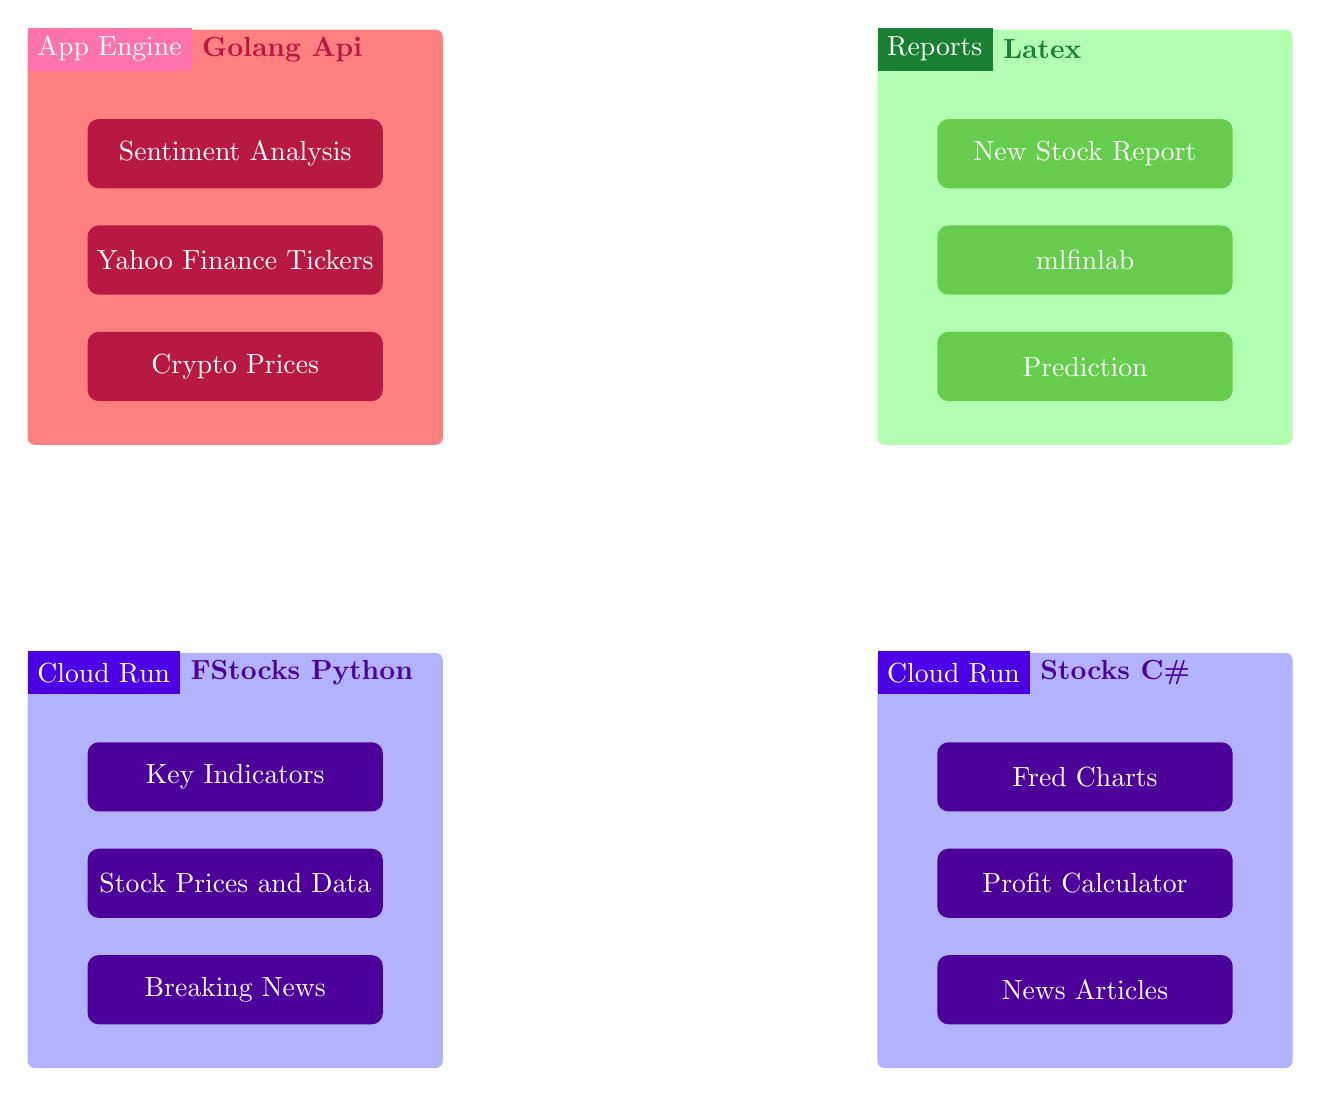
\begin{tikzpicture}
% Invisible reference center node
\node[draw=none] (stock-arch) {};
% Cloud stocks
\node[rectangle, rounded corners=0.25em,draw=none, minimum width=15em, minimum height=15em, fill=blue!30] (fstocks) at ([xshift=-15em] stock-arch.west) {};
% Needed to adjust the yshift to get it perfectly positioned
\node[sectionHeader={cloudrunMain}, yshift=-0.725em, anchor=west] (title) at (fstocks.north west)        {\nodepart[color=white]{one} Cloud Run
        \nodepart{two} \textcolor{cloudrunSecond}{\textbf{FStocks Python}}};

\node[coloredBox={10em}{2.5em}{10em}{cloudrunSecond}, yshift=-4.5em, line width=0.01pt] (fstocks-key) at (fstocks.north) {Key Indicators};
\node[coloredBox={10em}{2.5em}{10em}{cloudrunSecond}, yshift=-1em, below of = fstocks-key, line width=0.01pt] (fstocks-data)  {Stock Prices and Data};
\node[coloredBox={10em}{2.5em}{10em}{cloudrunSecond}, yshift=-1em, below of = fstocks-data, line width=0.01pt] (fstocks-news)  {Breaking News};

% Google Cloud C# stocks
\node[rectangle,rounded corners=0.25em,draw=none, minimum width=15em, minimum height=15em, fill=blue!30] (stocks-app) at ([xshift=15em] stock-arch.east) {};
% Needed to adjust the yshift to get it perfectly positioned
\node[sectionHeader={cloudrunMain}, yshift=-0.725em, anchor=west] (title) at (stocks-app.north west)        {\nodepart[color=white]{one} Cloud Run
        \nodepart{two} \textcolor{cloudrunSecond}{\textbf{Stocks C\#}}};
\node[coloredBox={10em}{2.5em}{10em}{cloudrunSecond}, yshift=-4.5em, line width=0.01pt] (stocks-app-data) at (stocks-app.north) {Fred Charts};
\node[coloredBox={10em}{2.5em}{10em}{cloudrunSecond}, yshift=-1em, below of = stocks-app-data, line width=0.01pt] (stocks-app-profit)  {Profit Calculator};
\node[coloredBox={10em}{2.5em}{10em}{cloudrunSecond}, yshift=-1em, below of = stocks-app-profit, line width=0.01pt] (stocks-app-news)  {News Articles};

% GAE Golang library switch colours
\node[rectangle,rounded corners=0.25em,draw=none, minimum width=15em, minimum height=15em, fill=red!50] (gae-server) at ([yshift=15em] fstocks.north) {};
% Needed to adjust the yshift to get it perfectly positioned
\node[sectionHeader={appengineMain}, yshift=-0.725em, anchor=west] (title) at (gae-server.north west)        {\nodepart[color=white]{one} App Engine
        \nodepart{two} \textcolor{appengineSecond}{\textbf{Golang Api}}};
\node[coloredBox={10em}{2.5em}{10em}{appengineSecond}, yshift=-4.5em, line width=0.01pt] (gae-server-data) at (gae-server.north) {Sentiment Analysis};
\node[coloredBox={10em}{2.5em}{10em}{appengineSecond}, yshift=-1em, below of = gae-server-data, line width=0.01pt] (gae-server-profit)  {Yahoo Finance Tickers};
\node[coloredBox={10em}{2.5em}{10em}{appengineSecond}, yshift=-1em, below of = gae-server-profit, line width=0.01pt] (gae-server-news)  {Crypto Prices};

% GAE Golang library switch colours
\node[rectangle,rounded corners=0.25em,draw=none, minimum width=15em, minimum height=15em, fill=green!30] (reports) at ([yshift=15em] stocks-app.north) {};
% Needed to adjust the yshift to get it perfectly positioned
\node[sectionHeader={reportsMain}, yshift=-0.725em, anchor=west] (title) at (reports.north west)        {\nodepart[color=white]{one} Reports
        \nodepart{two} \textcolor{reportsMain}{\textbf{Latex}}};
\node[coloredBox={10em}{2.5em}{10em}{reportsSecond}, yshift=-4.5em, line width=0.01pt] (reports-new) at (reports.north) {New Stock Report};
\node[coloredBox={10em}{2.5em}{10em}{reportsSecond}, yshift=-1em, below of = reports-new, line width=0.01pt] (reports-mlfinlab)  {mlfinlab};
\node[coloredBox={10em}{2.5em}{10em}{reportsSecond}, yshift=-1em, below of = reports-mlfinlab, line width=0.01pt] (reports-prediction)  {Prediction};

\end{tikzpicture}
\end{document}